% ----------------------------------------------------------


\chapter[Fundamentação Teórica]{Fundamentação Teórica}\label{Fundamentacao}
\begin{enumerate}
   \item  Como contribuição teórica inicial para o nosso projeto, temos o material do canal no Youtube 'Python Engineer' a playlist de vídeo aulas,  'Chat Bot With PyTorch - NLP Beginner Tutorial' \footnote{\url{https://www.youtube.com/playlist?list=PLqnslRFeH2UrFW4AUgn-eY37qOAWQpJyg}}. A partir desse conteúdo poderemos dar início aos nossos desenvolvimentos e pesquisas. No tutorial, é desenvolvido um chatbot simples usando PyTorch e Deep Learning. Também fornecendo uma introdução a algumas técnicas básicas de Processamento de Linguagem Natural (PLN).

   \item Seguiremos, também, os conteúdos já aprendidos nas aulas de  'Inteligência Artifical 2022/2 - UENF' para nos auxiliar na formulação teórica do nosso projeto.

   \item  Salientamos que com o decorrer do projeto nossas referências de materiais, para esse projeto, tenderá a aumentar devido a novas descobertas.
\end{enumerate}







\chapter[Metodologia]{Metodologia}

Baseado no “Project-based learning” \cite{krajcik2006project}. Seguiremos os estudos através de um projeto que aborda problemas do mundo real, cujo muitos não tem resposta única. Ao longo desse projeto será possível fazer novas perguntas e encontrar suas possíveis respostas por meio de uma investigação sustentada.

\justifying
\vspace {1mm}

Este Plano de Pesquisa também utilizará as seguintes metodologias:
\begin{itemize}
   \item \textit{Pesquisa Exploratória; visando promover o enriquecimento do conhecimento sobre os diferentes assuntos relacionados a IA, ML, e Chatbots:
         }
         \begin{itemize}
            \item \textit{Levantamento Bibliográfico;}
            \item \textit{Levantamento documental;}
            \item \textit{Minicursos e Vídeo aulas;}
            \item \textit{Obtenção de experiências.}
         \end{itemize}
\end{itemize}

\chapter[Construindo um Chatbot com Pytorch]{Construindo um Chatbot com Pytorch}

Já pensou em como Alexa, Siri ou assistente de voz do Google funcionavam? Neste capítulo daremos início à construção de um chatbot para interação com usuários de uma loja virtual.

Antes de continuar, abaixo encontra-se a lista de requisitos para o nosso projeto:
\justifying
\begin{itemize}
   \item \textit{Python 3}
         \begin{itemize}
            \item \textit{Define: Python} é uma linguagem de programação interpretada, orientada a objetos e de alto nível com semântica dinâmica. Suas estruturas de dados embutidas de alto nível, combinadas com tipagem dinâmica e vinculação dinâmica, o tornam muito atraente para o Desenvolvimento Rápido de Aplicativos e para uso como uma linguagem de script ou cola para conectar componentes existentes \footnote{\url{https://www.python.org/doc/essays/blurb/}}.
         \end{itemize}

   \item \textit{Dictionaries e Lists}
         \begin{itemize}
            \item \textit{Define: Listas} são tipos de dados mutáveis em Python. Lists é um tipo de dados de índice baseado em 0, o que significa que o índice do primeiro elemento começa em 0. As listas são usadas para armazenar vários itens em uma única variável. As listas são um dos 4 tipos de dados do Python, ou seja, Listas, Dicionário, Tupla e Conjunto \footnote{\url{https://www.analyticsvidhya.com/blog/2021/06/working-with-lists-dictionaries-in-python/}}.
            \item \textit{Define: Dicionários} Dicionários são a implementação do Python de uma estrutura de dados que é mais conhecida como uma matriz associativa. Um dicionário consiste em uma coleção de pares chave-valor. Cada par de chave-valor mapeia a chave para seu valor associado\footnote{\url{https://realpython.com/python-dicts}}.
         \end{itemize}

   \item \textit{NumPy}
         \begin{itemize}
            \item \textit{Define: NumPy} é o pacote fundamental para computação científica em Python. É uma biblioteca Python que fornece um objeto array multidimensional, vários objetos derivados (como arrays e matrizes mascarados) e uma variedade de rotinas para operações rápidas em arrays, incluindo matemática, lógica, manipulação de formas, classificação, seleção, E/S , Fourier discreto transforma álgebra linear básica, operações estatísticas básicas, simulação aleatória e muito mais\footnote{\url{https://numpy.org/doc/stable/user/whatisnumpy.html}}.
         \end{itemize}

   \item \textit{Pandas}
         \begin{itemize}
            \item \textit{Define: Pandas} é um pacote Python de código aberto que é mais amplamente usado para ciência de dados/análise de dados e tarefas de aprendizado de máquina. Ele é construído em cima de outro pacote chamado Numpy, que fornece suporte para arrays multidimensionais\footnote{\url{https://www.activestate.com/resources/quick-reads/what-is-pandas-in-python-everything-you-need-to-know/}}.
         \end{itemize}

   \item \textit{Pytorch}
         \begin{itemize}
            \item \textit{Define: PyTorch} é uma biblioteca de aprendizado de máquina para Python usada principalmente para processamento de linguagem natural. O software de código aberto foi desenvolvido pelas equipes de inteligência artificial do Facebook Inc. em 2016. O PyTorch oferece dois recursos significativos, incluindo computação de tensor, bem como redes neurais profundas funcionais\footnote{\url{https://deepai.org/machine-learning-glossary-and-terms/pytorch}}.
         \end{itemize}

   \item \textit{Natural Language Processing (Bag of Words)}
         \begin{itemize}
            \item \textit{Define: NLP ou PLN }O processamento de linguagem natural usa aprendizado de máquina para revelar a estrutura e o significado do texto. Com aplicativos de processamento de linguagem natural, as organizações podem analisar texto e extrair informações sobre pessoas, lugares e eventos para entender melhor o sentimento da mídia social e as conversas com os clientes \footnote{\url{https://cloud.google.com/learn/what-is-natural-language-processing}}.
         \end{itemize}


\end{itemize}

\section[Importando Bibliotecas Relevantes]{Importando Bibliotecas Relevantes}
\begin{lstlisting}[language=Python, caption=Python Bibliotecas]

   import numpy as np
   import random
   import json
   import nltk
   import torch
   import torch.nn as nn
   from torch.utils.data import Dataset, DataLoader
\end{lstlisting}


\section[Criando funções personalizadas]{Criando funções personalizadas}
Criaremos funções personalizadas para que seja fácil implementá-las posteriormente.
\justifying
\begin{lstlisting}[language=Python, caption=Python Funções personalizadas]
def tokenize(sentence):
    return nltk.word_tokenize(sentence)

def stem(word):
    return stemmer.stem(word.lower())

\end{lstlisting}
Nltk ou kit de ferramentas de linguagem natural é uma biblioteca realmente útil que contém classes importantes que serão úteis em qualquer uma de suas tarefas de PNL.
\justifying
\section[Stemming]{Stemming}


Se tivermos as seguintes palavras como Andei, Ande, Andarei, Andamento, Andando, Andante, podem parecer palavras diferentes, mas geralmente têm o mesmo significado e também a mesma forma base; "and".
O processo de stemização (do inglês, stemming) consiste em reduzir uma palavra ao seu radical. A palavra “meninas” se reduziria a “menin”, assim como “meninos” e “menininhos”. As palavras “gato”, “gata”, “gatos” e “gatas” reduziriam-se para “gat” \footnote{\url{https://www.computersciencemaster.com.br/como-reduzir-uma-palavra-ao-seu-radical-em-python-stemming/}}.
Então, para que nosso modelo entenda todas as formas diferentes das mesmas palavras, precisamos treinar nosso modelo com essa forma. Isso é chamado de Stemming. Existem diferentes métodos que podemos usar para derivação. Aqui usaremos o modelo Porter Stemmer da nossa biblioteca NLTK.
\justifying
\begin{lstlisting}[language=Python, caption=Python Stemming]
from nltk.stem.porter import PorterStemmer
stemmer = PorterStemmer()
\end{lstlisting}

\section[Bag of Words]{Bag of Words}
Vamos dividir cada palavra em frases e adicioná-la a um array. Nós estaremos usando um saco de palavras. Que inicialmente será uma lista de zeros com um tamanho igual ao comprimento do array all-words. Se tivermos um array de ` frases = ["ola", "como", "voce", "esta"]` e um array de total ` words = ["oi", "olá", "eu", "você, "tchau", "obrigado", "legal"]` então seu conjunto de palavras será `bog = [ 0 , 1 , 0 , 1 , 0 , 0 , 0]`. Faremos um loop sobre cada palavra no array all-words e o array bog correspondente a cada palavra. Se uma palavra da frase for encontrada no array all words, 1 será substituído naquele índice/posição no array bag.
\justifying


\begin{figure}[H]
   \begin{center}
      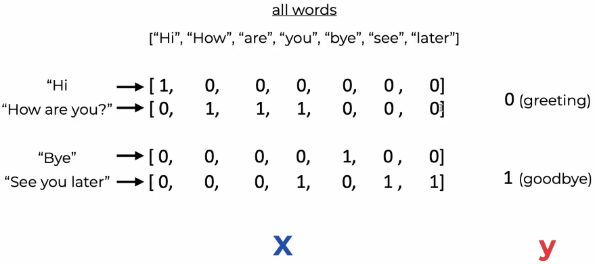
\includegraphics[width=15cm]{img/bagofwords.png}
      \caption{Bag of Words} \label{BagofWords}
      \medskip
      \small
      Usa Bag of Words para separar uma frase em várias palavras. Imagem retirada da Fundamentação Teórica \ref{Fundamentacao}.
   \end{center}
\end{figure}


\begin{lstlisting}[language=Python, caption=Python Bag of Words]
def bag_of_words(tokenized_sentence, words):
    """
    return bag of words array:
    1 para cada palavra conhecida que existe na frase,
    0 caso contrario.


    Exem,plo:


    sentence = ["ola", "como", "esta", "voce"]
    words = ["oi", "ola", "eu", "voce", "tchau",
     "obrigado", "legal"]
    bag   = [  0 ,    1 ,    0 ,   1 ,    0 ,    0 ,      0]
    """
    # stem cada palavra
    sentence_words = [stem(word) for word in tokenized_sentence]
    # initialize bag com 0 para cada palavra
    bag = np.zeros(len(words), dtype=np.float32)
    for idx, w in enumerate(words):
        if w in sentence_words:
            bag[idx] = 1

    return bag

\end{lstlisting}

Durante o processo, também usaremos \textbf{nltkwordtokenize()} que converterá uma única string de sentença em uma lista de palavras. Por exemplo, se você passar \textbf{"Ola, como voce esta?"}, ele retornará \textbf{"ola", "como", "voce", "esta"}.
\textbf{Observação:} Passaremos palavras em minúsculas para o \textbf{Stemmer} para que palavras como Bom e bom (em maiúsculas) não sejam rotuladas como palavras diferentes.

\section[Carregando os dados e Data Cleaning]{Carregando os dados e Data Cleaning}
Usaremos um conjunto de dados chamado  \textbf{intents.json} que tem a estrutura mostrada no campo abaixo. Estaremos limpando esses dados de acordo com as nossas necessidades usando as funções que criamos anteriormente.

\begin{lstlisting}[language=python, caption=Data intents.json]
{
  "intents": [
    {
      "tag": "saudacao",
      "patterns": [
        "Oi",
        "Ei",
        "Como voce esta",
        "Tem alguem ai?",
        "Ola",
        "Bom dia"
      ],
      "responses": [
        "Ei :-)",
        "Ola, obrigado pela visita",
        "Ola, o que posso fazer por voce?",
        "Ola, como posso ajudar?"
      ]
   }
  ]
}


\end{lstlisting}
Agora vamos simplesmente carregar o arquivo json usando a função \textbf{jsonload}.

\begin{lstlisting}[language=Python, caption=Python Carregando dados]
with open('intents.json', 'r') as f:
    intents = json.load(f)
\end{lstlisting}

Para obter as informações corretas, iremos descompactá-las com o seguinte código:

\begin{lstlisting}[language=Python, caption=Python Loop nos dados]
all_words = []
tags = []
xy = []
# loop atraves de cada frase no nosso intents patterns
for intent in intents['intents']:
    tag = intent['tag']
    # adicionar a tag list
    tags.append(tag)
    for pattern in intent['patterns']:
        # tokenize cada palavra na frase
        w = tokenize(pattern)
        # adicionar a nossa lista de palavras
        all_words.extend(w)
        # adicionar ao par xy
        xy.append((w, tag))

\end{lstlisting}
Isso separará todas as tags e palavras em suas listas.

\section[Limpeza e preparação dos dados]{Limpeza e preparação dos dados}


Estaremos usando nossas funções personalizadas e limpando os dados implementando as funções que criamos em nossas células anteriores.

\begin{lstlisting}[language=Python, caption=Data Cleaning]

# stem e lower cada palavra
ignore_words = ['?', '.', '!']
all_words = [stem(w) for w in all_words if w not in ignore_words]
# remover duplicados e sort
all_words = sorted(set(all_words))
tags = sorted(set(tags))

print(len(xy), "patterns") # padroes
print(len(tags), "tags:", tags) # tags
print(len(all_words), "unique stemmed words:", all_words) # palavras derivadas unicas

\end{lstlisting}

Criando dados de treinamento: transformaremos os dados em um formato que nosso modelo PyTorch possa entender facilmente

\begin{lstlisting}[language=Python, caption=Training Data]

# criar dados de treinamento
X_train = []
y_train = []
for (pattern_sentence, tag) in xy:
    # X: bag de palavras para cada pattern_sentence
    bag = bag_of_words(pattern_sentence, all_words)
    X_train.append(bag)
    # y: PyTorch CrossEntropyLoss precisa apenas class labels, nao one-hot
    label = tags.index(tag)
    y_train.append(label)

X_train = np.array(X_train)
y_train = np.array(y_train)

\end{lstlisting}

\section[Modelo PyTorch]{Modelo PyTorch}

Aqui estaremos fazendo uma classe para implementar nossa rede neural personalizada. Será uma Rede neural feed-forward que terá 3 Camadas Lineares e usaremos a função de ativação “ReLU”. Nota: Usamos a função super() para herdar as propriedades de sua classe pai. Este é um conceito de Programação Orientada a Objetos (OOP).

\begin{itemize}
   \item \textit{Define: ReLU} é uma função de ativação não linear que é usada em redes neurais multicamadas ou redes neurais profundas. Esta função pode ser representada como:

         \begin{figure}[H]
            \begin{center}
               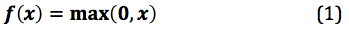
\includegraphics[width=10cm]{img/relu.jpg}
               \caption{ReLu} \label{ReLu}
               \medskip
               \small
               onde x = um valor de entrada.
            \end{center}
         \end{figure}

         De acordo com a equação 1, a saída de ReLu é o valor máximo entre zero e o valor de entrada. A saída é igual a zero quando o valor de entrada é negativo e o valor de entrada quando a entrada é positiva. Assim, podemos reescrever a equação 1 da seguinte forma:

         \begin{figure}[H]
            \begin{center}
               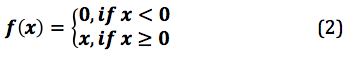
\includegraphics[width=10cm]{img/relu2.jpg}
               \caption{ReLu} \label{ReLu2}
               \medskip
               \small
               onde x = um valor de entrada.
            \end{center}
         \end{figure}


         Exemplos de ReLu: Dadas diferentes entradas, a função gera diferentes saídas. Por exemplo, quando x é igual a -5, a saída de f(-5) é 0. Por outro lado, a saída de f(0) é 0 porque a entrada é maior ou igual a 0. Além disso, o resultado de f (5) é 5 porque a entrada é maior que zero \footnote{\url{https://deepai.org/machine-learning-glossary-and-terms/relu/}}.
\end{itemize}

\subsection[Feed Forward Neural Network]{Feed Forward Neural Network}

\textit{Define: Feed Forward Neural Network} Uma Rede Neural Feed Forward é uma rede neural artificial na qual as conexões entre os nós não formam um ciclo. O oposto de uma rede neural feed-forward é uma rede neural recorrente, na qual certos caminhos são ciclados. O modelo feed-forward é a forma mais simples de uma rede neural, pois a informação é processada apenas em uma direção. Embora os dados possam passar por vários nós ocultos, eles sempre se movem em uma direção e nunca para trás \footnote{\url{https://deepai.org/machine-learning-glossary-and-terms/feed-forward-neural-network}}.


\begin{figure}[H]
   \begin{center}
      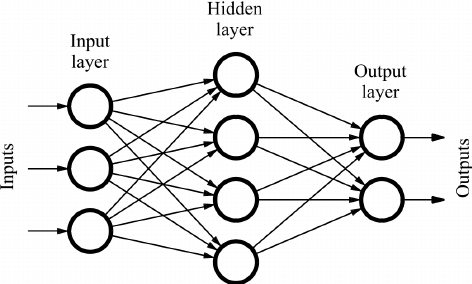
\includegraphics[width=10cm]{img/ffnn.png}
      \caption{Feed Forward Neural Network} \label{ffnn}
      \medskip
      \small
      Exemplo de uma rede neural feed-forward.
   \end{center}
\end{figure}

Desse modo, uma representação válida para o nosso projeto seria a FFNN abaixo:
\begin{figure}[H]
   \begin{center}
      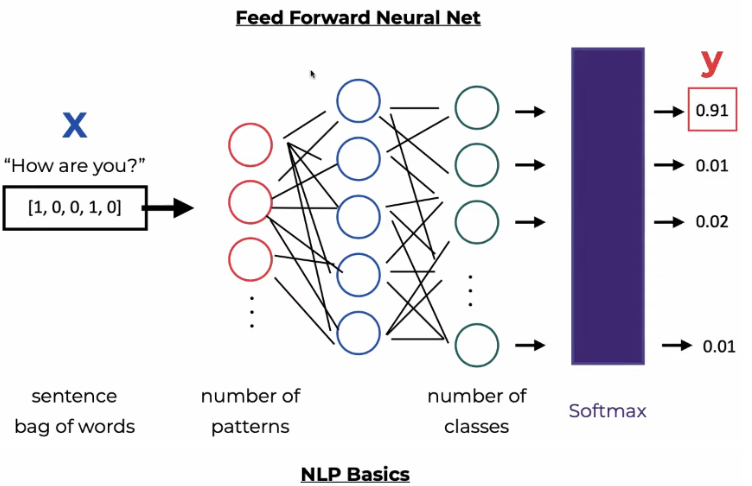
\includegraphics[width=10cm]{img/ffnn2.png}
      \caption{Feed Forward Neural Network} \label{ffnn2}
      \medskip
      \small
      Exemplo de uma rede neural feed-forward para o nosso projeto. Imagem retirada da Fundamentação Teórica \ref{Fundamentacao}.
   \end{center}
\end{figure}
